%!TeX root = ../main.tex


\section{Conclusions}
By performing a reconstruction in COLMAP, a final result is obtained and in this case, as shown in fig. \ref{fig:fountaintrue} and \ref{fig:tisotrue}, the fountain is rebuilt in a more sparse form due to the smaller amount of information provided to the software. In fact, from the statistics, there is a mean of observations per image equal to 4751.36 and a total number of observations equal to 52256. The data are almost a third lower than those obtained with the SURF algorithm without using the compression of the descriptors. Fig. \ref{fig:fountainautoenc} and \ref{fig:tisoautoenc} refers precisely to the final result without the use of the autoencoder and therefore all the features and matchings obtained by the SURF algorithm are supplied to COLMAP without regression. Comparing the two results, significant differences are visible in the reconstruction quality of the fountain.


\begin{figure}[H]
     \centering
     \begin{subfigure}[b]{.5\textwidth}
		\centering
		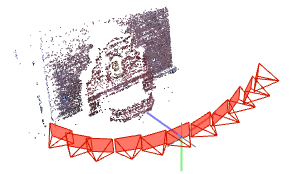
\includegraphics[width=\textwidth]{images/fountainautoenc.png}  
		\caption{\centering Fountain reconstructed with the autoencoder.}
	    	\label{fig:fountainautoenc} 
     \end{subfigure}
     \hfill
     \begin{subfigure}[b]{0.49\textwidth}
		\centering
    		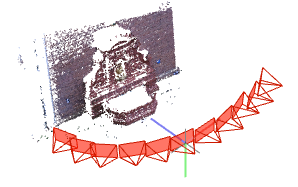
\includegraphics[width=\textwidth]{images/fountaintrue.png}
		\caption{\centering Fountain reconstructed without the autoencoder.}
		\label{fig:fountaintrue}   
     \end{subfigure}
        \caption{Fountain reconstruction using COLMAP.}
        \label{fig:fountain3D}
\end{figure}


\begin{figure}[H]
     \centering
          \begin{subfigure}[b]{0.5\textwidth}
		\centering
    		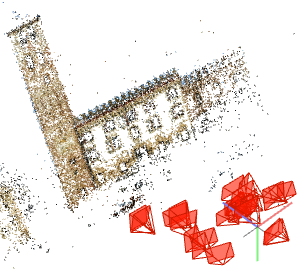
\includegraphics[width=\textwidth]{images/tisoautoenc.png}
		\caption{\centering Tiso reconstructed with the autoencoder.}
		\label{fig:tisoautoenc}   
     \end{subfigure}
     \hfill
     \begin{subfigure}[b]{.49\textwidth}
		\centering
		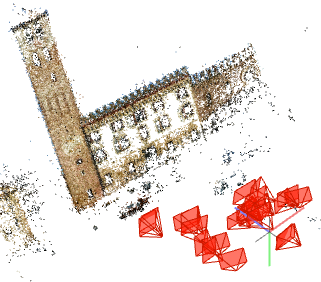
\includegraphics[width=\textwidth]{images/tisotrue.png}  
		\caption{\centering Tiso reconstructed without the autoencoder.}
	    	\label{fig:tisotrue} 
     \end{subfigure}
        \caption{Tiso reconstruction using COLMAP.}
        \label{fig:Tiso3D}
\end{figure}


This type of compression can be useful in environments where the quality of reconstruction is not important, for example in object detection, where is not crucial to exactly reconstruct the object with respect to the detection result ``true/false''. In can be seen from the compressed images that the edges of the objects are mostly preserved while straight planes are ``thinned out'', i.e. represented with less points.